\section{Photon beam flux}

\subsection{Photon beam flux accounting with the GlueX pair spectrometer}
The photon beam flux can be directly extracted by analyzing the pair
spectrometer (PS) data with the thin beryllium converter installed in
the beam in from of it.  The absolute normalization of the PS
performed with the total absorption counter (TAC) during the dedicated
run.

The systematics from the photon beam flux accounting by pair
spectrometer is originated from few main contributions: overall
spectrometer calibration with TAC quality; accuracy of the Monte-Carlo
simulation of this process; long term stability of the spectrometer
performance; and change of conditions between low intensity beam (TAC
calibration) and production intensity.  There are few other less
significant contributions. GlueX PS acceptance \cite{hdnote3684} shown
on Fig.~\ref{fig:psacc}. For the proposed experiment PS magnetic field
should be reduced to cover the beam energy range $5-6\,GeV$.
\begin{figure}[tpb]
\begin{center}
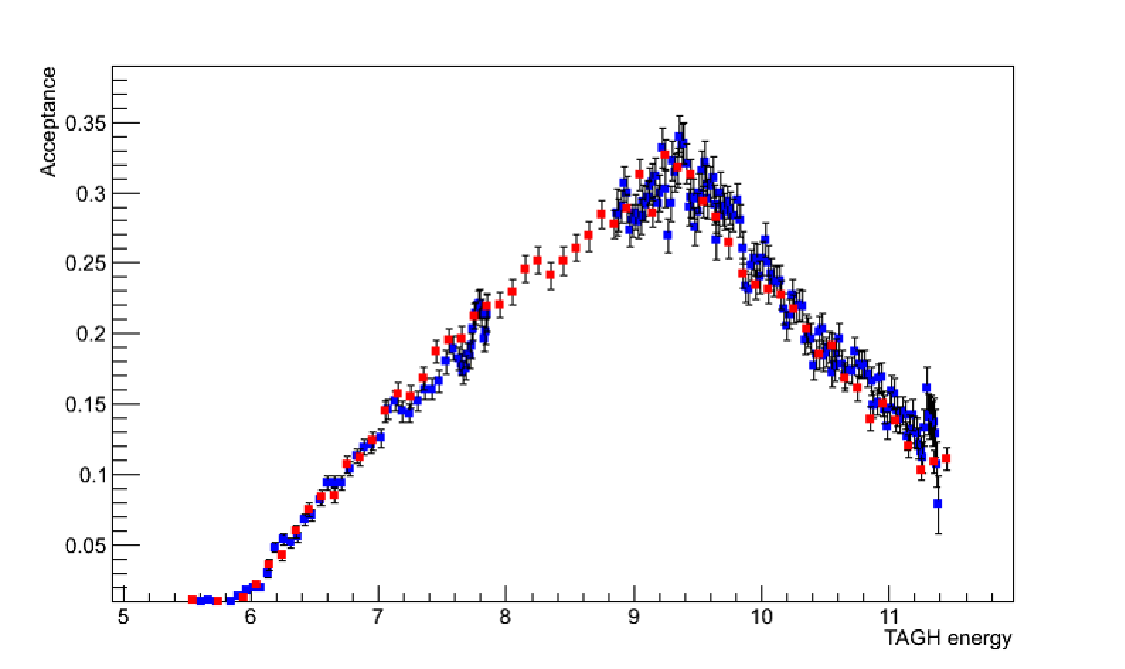
\includegraphics[width=10cm,angle=0]{figures/ps_acceptance.pdf}
\end{center}
\caption{GlueX PS acceptance extracted from TAC data analysis (blue points);
red points -- Monte-Carlo simulation}
\label{fig:psacc}
\end{figure}
The methodology and accuracy of the PS analysis is the same as in
PrimEx-D experiment, currently running in Hall-D, and has value
$\sim1-1.5\,\%$ \cite{PrimexDexp}.

\subsection{Cross section verification with the exclusive single $\pi^0$ photoproduction}
The extracted cross section can also be normalized on or independently
from PS analysis verified with the $\pi^0$ radiative decay width
extraction.  Fig.~\ref{fig:leaddndt} shows exclusive single $\pi^0$
photoproduction yield at forward angle obtained by the PrimEx
experiment and used for $\pi^0$ radiative decay width extraction.
\begin{figure}[tpb]
\begin{center}
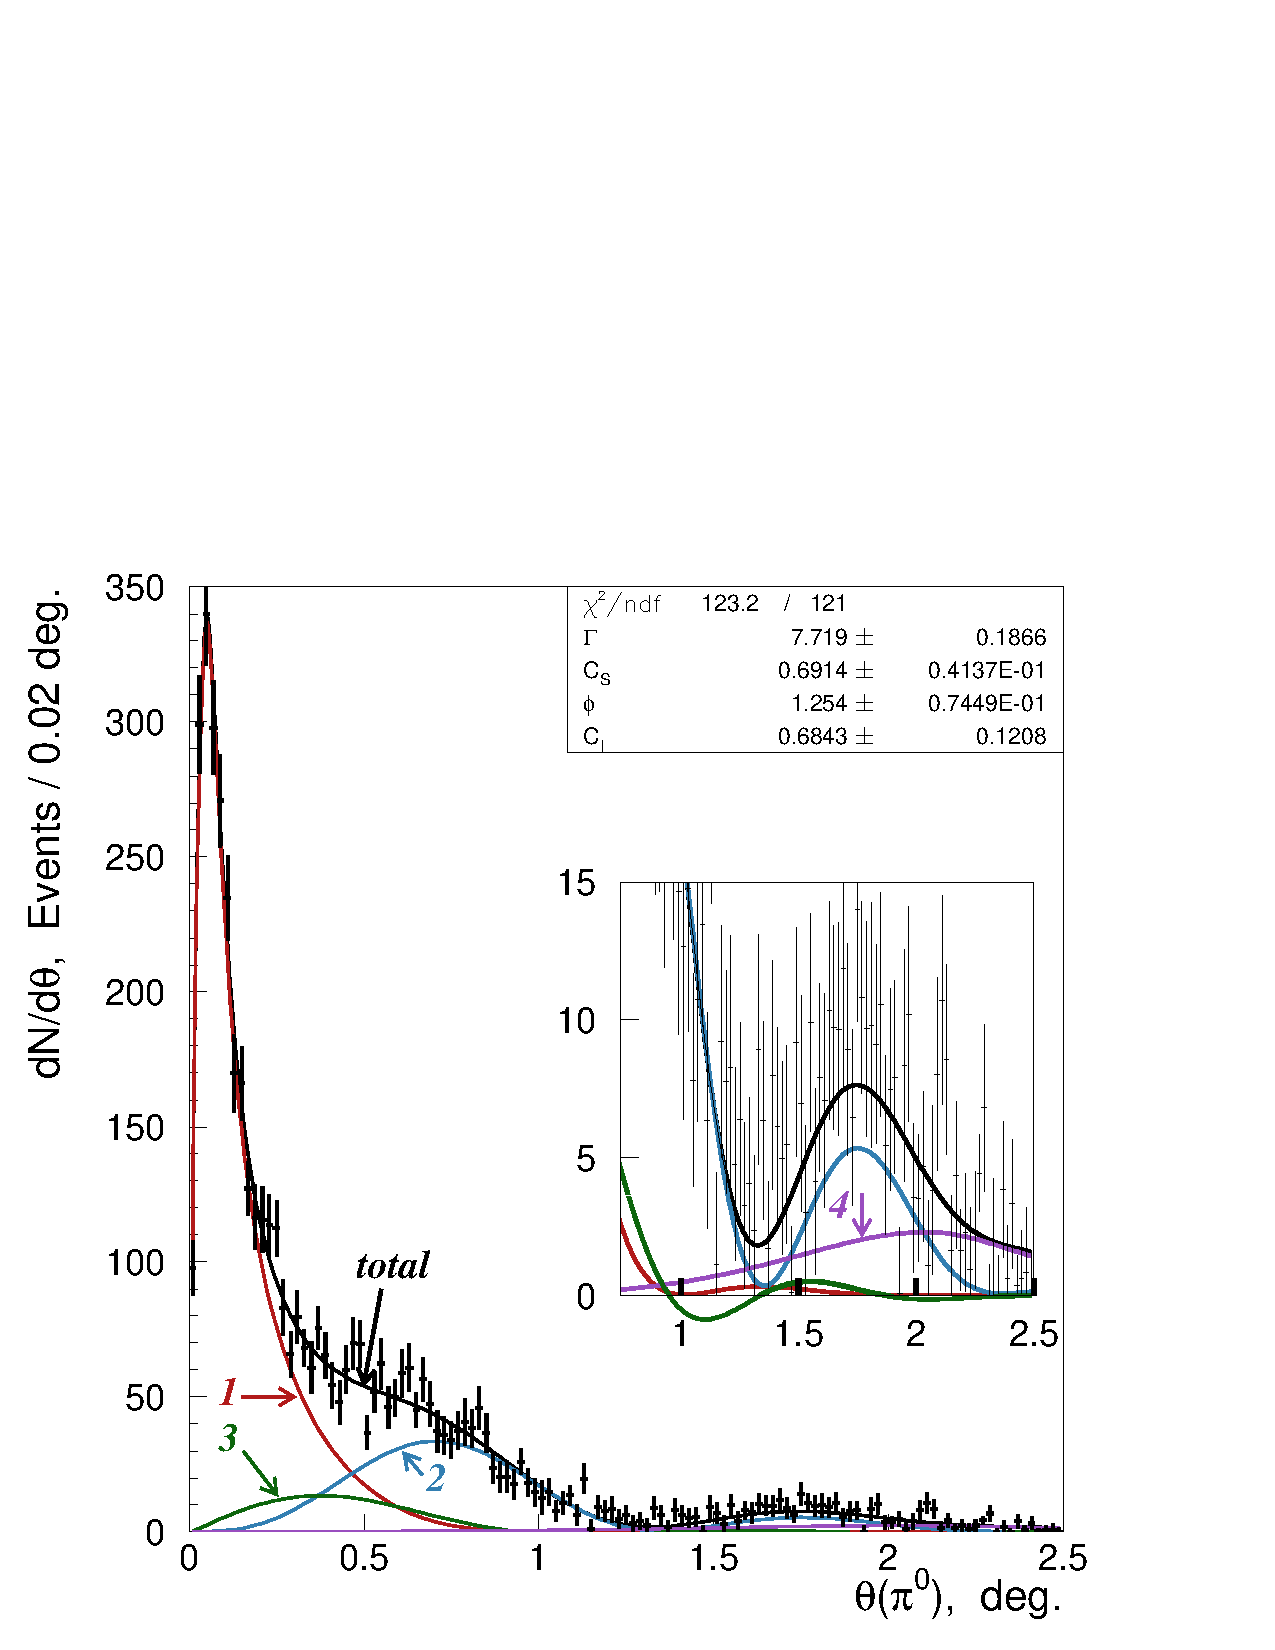
\includegraphics[width=8cm,angle=0,trim={1.5cm 0.5cm 3.5cm 9.5cm},clip]{figures/dndt_pb_partial.pdf}
\end{center}
\caption{Exclusive $\pi^0$ production yield at forward angle on lead target
observed in the PrimEx experiment \cite{Larin:2010kq}. Curves show production mechanisms input:
1 -- Primakoff, 2 -- strong coherent, 3 -- interference of first two mechanisms, 4 -- strong incoherent}
\label{fig:leaddndt}
\end{figure}
The photon beam flux in PrimEx was $0.725\times10^{12}$ for
4.9-5.5$\,$GeV bremsstrahlung spectrum part on 5\% rad. len. lead
target. The distance between calorimiter and target was $\sim7.3\,m$
and the central square part of the calorimeter, used in analysis was
$\sim70\times70\,cm$. These conditions have to be compared with the
proposed experiment conditions: 20 days of $~10^7$ collimated beam
photon/sec (i.e. 20 times more than PrimEx lead target beam flux), the
distance between target and FCAL $\sim6.2\,m$ and active calorimeter
part diameter $\sim2\,m$.  The central hole with one calorimeter
modules layer around which should be excluded from the analysis for
PrimEx case was $\sim8\times8\,cm$ and for FCAL $\sim20\times20\,cm$,
which is decreasing FCAL acceptance at forward angle. Comparison of
these experimental conditions allows us expecting an order of
magnitude higher exclusive single $\pi^0$ photoproduction statistics.
Thus PrimEx statistical uncertainty for lead will be decreased from
$\sim2.5\,\%$ down to $\sim1\,\%$.  For the systematical uncertainty,
in PrimEx it was $\sim2.1\,\%$ and has two major contributions: yield
extraction ($\sim1.6\,\%$) and photon beam flux accounting
($\sim1.0\,\%$).  The first contribution is partly statistically
driven and reduces with increasing of statistics; and the second one
cancels out since it is the same photon beam flux for the single and
double exclusive $\pi^0$ photoproduction.  The main factors increasing
systematics for the proposed experiment are: the angular resolution of
FCAL is about a factor of two worse than for PWO crystals used in the
PrimEx analysis;
%the single $\pi^0$ photoproduction theory needs to be involved since
%the photon beam energy spectra are not the same for PrimEx and
%proposed experiment;
and the magnetic field is not swiping out charged background like it
was in PrimEx.  As a result we can expect slightly worse systematical
uncertainty than in PrimEx and statistical precision of $\sim1\,\%$,
i.e. total error $2.5-3.5\,\%$ for $\pi^0$ radiative width extraction
(excluding absolute photon beam flux accounting, target number of
atoms and partly FCAL trigger efficiency contributions to the
systematics which are canceling out).  The expected total beam flux
uncertainty for such a normalization should also include the PrimEx
total error of the $\pi^0$ radiative width, which was recently
reported as 1.5\% \cite{Larin:2018}.  All this gives $\sim3-4\,\%$
error for photon beam flux from normalization to the re-extracted $\pi^0$ radiative decay width.

\subsection{Muon pair production}
In addition to these normalization channels, production of muon pairs,
which has a known cross section, can be used as a measurement of
photon flux. Since the experiment will be running concurrently with
the Charged Pion Polarizability (CPP) experiment, the photon flux on
target will be the same by definition. CPP plans to use muon pair
creation by beam photons as its main normalization channel, and so
those measurements will be available for normalization of the neutral
pion channel as well. In the case of CPP, the GlueX track finding and
fitting efficiency will have to be determined for muon pairs, but any
systematic error in that determination will largely cancel when
applied to charged pion pairs. That will not be the case for the
neutral pion channel and will have to be taken into account when
evaluating systematic errors due to this method of normalization. In
any case, muon pair production should provide a useful check on the
other methods mentioned above.
